\documentclass[12pt]{IEEEtran}
\usepackage[utf8]{inputenc}
\usepackage{graphicx}
\usepackage{amsmath, amsthm, amssymb}

\title{Chaos Project 1}
\author{
  Paul Booth \\
  \and
  Geoff Pleiss
}
\date{}

\newtheorem{thm}{Theorem}
\newtheorem{lma}{Lemma}

\begin{document}
  \maketitle

\begin{abstract}
\end{abstract}



\section{Introduction}
% TODO: add to the introduction

The theorem we are trying to prove is

\begin{thm}
\label{thm:mainthm}
	Let $J$ be an interval and let $F$ be a continuous first-order map with $F : J \rightarrow J$. If there is some point $a \in J$ that satisfies the following
	%
	\[ F^3\left(a\right) \leq a < F\left(a\right) < F^2\left(a\right) \]
	or
	\[ F^3\left(a\right) \geq a > F\left(a\right) > F^2\left(a\right) \]
	%
	then $J$ contains a $k$-period orbit for all $k \in \mathbb{N}$.
\end{thm}

In the first section we will provide a rough outline of the proof for this theorem, which will be followed by the proof in full. We will then discuss the interpretations and implications of our results.



\section{The big picture}

In order to prove that a first-order map $F$ contains an orbit with period $k$, there are two things we must prove. First, we must show that there is a fixed point on the $k^{th}$ return map of F. In other words, we must show that there is some $x \in J$ for which $F^k \left( x \right) = x$. To understand why this implies periodicity, let's examine $F^2k \left( x \right)$. This is simply equal to $F^k \left( F^k \left( x \right) \right) = F^k \left( x \right) = x$. A simple inductive proof will show that $F^n \left( x \right) = x$ whenever $n \equiv 0 \left(\mod k \right)$, thus showing that $x$ is a periodic point.

However, even if we find a fixed point $x$ of $F^k$, this does not imply that the periodicity of $x$ is $k$. For example, $x$ could also be a fixed point of $F^{k/2}$. Thus $2$ orbits of $F$ would be completed $k$ iterations of the function, and so the periodicity of $x$ would be $k/2$. To show that $x$ has periodicity of $k$, we must also show that $x$ is {\it not} a fixed point of $F^m$ for any $m < k$.

If we show that there is some $x \in J$ that meets these criteria for an arbitrary $k$, then we will have proven that $F$ has orbits of every periodicity.



\section{Lemmas}


% TODO: FIGURE OUT HOW WE WANT TO PRESENT THIS ACTUALLY

\begin{lma}
\label{lma:cont_comp}
	Let $G : I \rightarrow R$ be continuous, where $I$ is an interval. For any compact interval $J \subset G(I)$ there is a compact interval $Q \subset J$ such that $G(Q) = J$.
\end{lma}

\begin{figure}
	\begin{center}
		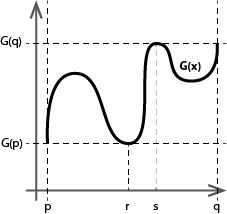
\includegraphics{img/continuity_graph.png}
		\caption{Diagram for Lemma \ref{lma:cont_comp}}
        \label{fig:continuity_graph}
	\end{center}
\end{figure}

{\it Proof}: Let $J = \left[ G \left( p \right), G \left( q \right) \right]$, where $p, q \in I$. If $p < q$, let $r$ be the last point of $\left[ p, q\right]$ where $G \left( r \right) = G \left( p \right)$ and let $s$ be the first point after $r$ where $G \left( s \right) = G \left( q \right)$, as shown in Figure \ref{fig:continuity_graph}. Then, $G \left( \left[ r, s\right] \right) = J = \left[ G \left( p \right), G \left( q \right) \right]$ as desired. Similar logic proves the $p > q$ case. $\Box$

% TODO: include why we use this lemma 0

\begin{lma}
\label{lma:fixedpoint}
	Let $F : J \rightarrow J$ and let $I \subseteq J$ be a compact interval such that $I \subseteq F \left( I \right)$. There exists at least one fixed point of F in the interval $I$ -- i.e. $x \in I$ such that $F \left( x \right) = x$.
\end{lma}

\begin{figure}
	\begin{center}
		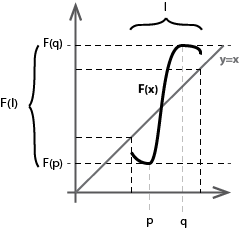
\includegraphics{img/fixedpoint_graph.png}
		\caption{Diagram for Lemma \ref{lma:fixedpoint}}
        \label{fig:fixedpoint_graph}
	\end{center}
\end{figure}

{\it Proof}: Define $p \in I$ such that $\min \left( F \left( I \right) \right) = F \left( p \right)$. Similarly, define $q \in I$ such that $\max \left( F \left( I \right) \right) = F \left( q \right)$ (see Figure \ref{fig:fixedpoint_graph}). Because $F \left( I \right) \supseteq I$, we know that $F \left( p \right) \leq p$ and $F \left( q \right) \geq q$. In other words, $F \left( p \right)$ would lie below the $y=x$ line, while $F \left( q \right)$ would like above the $y=x$ line. By continuity, there must be some point in between $p$ and $q$ that crosses the $y=x$ line, as can be seen in the figure. That is the fixed point of the function.

More formally, let $G \left( x \right) = F \left( x \right) - x$. Since $F \left( p \right) \leq p$ and $F \left( q \right) \geq q$, we know that $G \left( p \right) \leq 0$ and $G \left( q \right) \geq 0$. Since $G$ is continuous, we know by the Intermediate Value Theorem that there exists at least one $x$ such that $p \leq x \leq q$ and $G \left( x \right) = 0$. In other words, $F \left(x \right) = x$, making $x$ a fixed point of $F$. $\Box$



\section{The main theorem revisited}

Armed with the lemmas in the previous section, we are now ready to prove Theorem \ref{thm:mainthm}. Let $k$ be any natural number, let $F : J \rightarrow J$, and let $a \in J$ be the point in the assumptions of the theorem. Without loss of generality, let's assume that $F^3\left(a\right) \leq a < F\left(a\right) < F^2\left(a\right)$. (If the opposite is true, the proof follows the exact same steps). Let $b = F \left( a \right)$, $c = F ^2 \left( a \right)$, and $d = F^4  \left( a \right)$. Finally, let $L = \left[ b, c \right]$, and let $k = \left[ a,b \right]$.

%TODO: make sure that this proof works for the case where k=1

Again, the first step of showing that $F$ contains a $k$-cycle is to prove that $F^k$ has a fixed point $p_k \in J$. To do this, we will construct a set of nested intervals $I_n$  using Lemma \ref{lma:intervals}, which we will then apply Lemma \ref{lma:fixedpoint} to. Let $l_0$, $l_1$, $l_2$, $\cdots$, $l_{k-2}$ = $L$, and let $l_k$ = k. For $n \geq k$, we will let $I_n = I_l$, where $l = n \mod k$. Thus the intervals $I_n$ follow a repeating pattern. We will now show that for any $n \in \mathbb{N}$, $I_n \subseteq F \left( I_{n-1} \right)$. In the case where $I_n = I_{n-1} = L$, note that $F \left( b \right) = c$, and $F \left( c \right) = d < b$. By the Intermediate Value Theorem, $F$ must take on all values between $F \left( b \right)$ and $F \left( c \right)$ in the interval $L$. Therefore, $F \left( I_{n-1} \right) = F \left( L \right) = [d, c] \supset \left[ b,c \right] = L$. If $I_n = K = I_n$ and $I_{n-1} = L$, since $d \leq a$ we know that $F \left( I_{n-1} \right) = F \left( L \right) = [d, c] \supset \left[ a,b \right] = K = I_n$. Finally, in the case where $I_n = L$ and $I_{n-1} = K$, we know that $F \left( I_{n-1} \right) = F \left( K \right) = [a, b] = \left[ b,c \right] = L = I_n$. In all of these possible cases, note that $I_n \subseteq F \left( I_{n-1} \right)$ and thus $I_n$ fits the hypothesis of Lemma \ref{lma:fixedpoint}.
 


\section{Implications/Conclusions}

Though it appears that we have shown that there is some arbitrary number of fixed points of $F^k$, we can actually say a bit more about how many fixed points exist. Let $x_0$ be a point with periodicity of exactly $k$ for the function $F$.

Define $x_1$, $x_2$, $\cdots$, $x_{k-1}$ to be $F \left( x_0 \right)$, $F^2 \left( x_0 \right)$, $\cdots$, $F^{k-1} \left( x_0 \right)$, respectively. We know that $x_1$ cannot equal $x_0$ because otherwise the periodicity of $x$ would be less than $k$. We also know that $x_1$  cannot equal $x_2$, $x_3$, $\cdots$, $x_{k-1}$. Assume that there was some $l < k-1$ where $x_1 = x_l$. Then the sequence $x_n = F^n \left( x \right)$ would have terms $x_0$, $x_1$, $x_2$, $\cdots$, $x_l = x_1$, $x_2$, $\cdots$. Note that this sequence never returns to $x_0$, which would make $x_0$ a non-periodic point. Thus $x_1$ is a unique point, and it does not have periodicity less than $k$. A similar argument can be made for all the other points.

Now we can show that our $k$ points -- $x_0$, $x_1$, $\cdots$, $x_{k-1}$ -- are $k$-periodic. Given $x_l$, we know that $F^k \left( x_l \right) = F^{k+l} \left ( x_0 \right) = F^{l} \left ( x_0 \right) = x_l$. Thus we have shown that for each $l \in [0,k-1]$, $x_l$ is a unique point with periodicity of exactly $k$. Thus there are at least $k$ points that are $k$-periodic on the map $F$. If there was a $k+1^{th}$ unique $k$-periodic point, we could use a similar argument to show that there must be an additional $k-1$ more $k$-periodic points that lie on the $k+1^{th}$ point's orbit. To summarize, on any given map $F$ for which Theorem \ref{thm:maintheorem} applies, there are exatly $n \left( k \right)$ points with periodicity $k$, where $n \in \mathbb{N}$.

% TODO: include basic proof for how 3-cycle -> hypothesis
% TODO: add more implications

\end{document}

